\chapter{Known Issues}

\section{Assigning floating IP to gitlab-ce}

Assigning a floating IP to the gitlab-ce machine does not work in OpenStack and an error \ref{fig:floating_ip_error} is raised.

\begin{figure}[H]
	\centering
	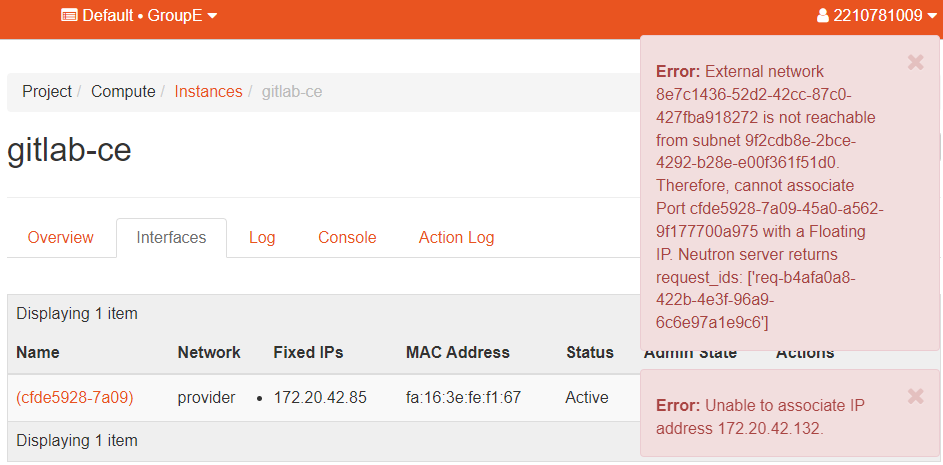
\includegraphics[width=14cm]{images/floating_ip_error.png}
	\caption{Error in OpenStack with floating IP assignment}
	\label{fig:floating_ip_error}
\end{figure}

To mitigate this issue, an IP from the DHCP pool can be used by just attaching the 'provider' network without setting a fixed IP. However, due to the issue described in \ref{leased_ip_gateway} this is no good solution, and it should be addressed on OpenStack level.

\section{Keeping leased IP and gateway} \label{leased_ip_gateway}

The machine 'gitlab-ce' looses its default gateway and sometimes even its leased IP after some time (single digit number of days).
This is very bad, because you not only cannot log in to GitLab via HTTPS, but you also cannot log in via SSH anymore to manage or analyze the whole thing.
But with a root password set to the machine, this can be verified on the OpenStack console.

\begin{figure}[H]
	\centering
	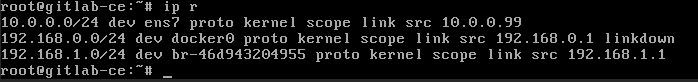
\includegraphics[width=14cm]{images/missing_ip_gateway.png}
	\caption{Missing default gateway}
	\label{fig:missing_ip_gateway}
\end{figure}

Up until now this can only be solved temporary by following these steps:
\begin{enumerate}
	\item Stop the machine
	\item Detach both network interfaces
	\item Attach only the 'provider' network (see \ref{gitlab_machine_network_configuration})
	\item Start the machine
	\item Verify SSH connection
	\item Also attach the 'gitlabrunners' network
\end{enumerate}

After following those steps, the machine should be fully functioning again and IP and routing information should look similar to \ref{fig:ip_gateway_ok}.

\begin{figure}[H]
	\centering
	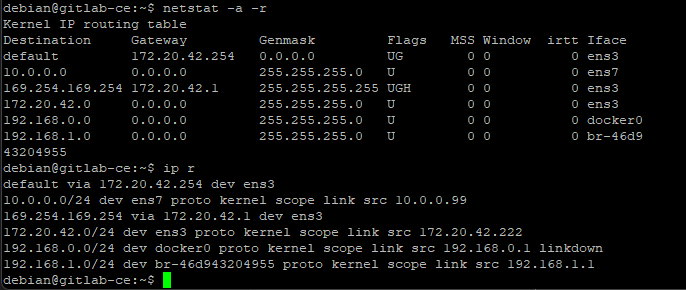
\includegraphics[width=14cm]{images/ip_gateway_ok.png}
	\caption{IP and routing information of working system}
	\label{fig:ip_gateway_ok}
\end{figure}